
\section{Problem}

The underlying mechanism enforcing CPU reservations for most modern containers
running on Linux is \cgroups{}' weight interface: all Open Container Initiative
(OCI) compliant containers, including Kubernetes, Docker, CRI-O, and containerd
use it~\cite{oci-cgroups, docker-docs-cgroups, container-isolation-article}, as
do VM frameworks, including Firecracker, AFaas and
libvirt~\cite{firecracker-cgroups,afaas,libvirt-cgroups}. Kubernetes for
instance creates one top level group for all BE services and assigns it the
lowest weight of 1, and pods with reservations are in separate groups with
higher weights, \eg{} in the experiment the server asked for 4 CPUs and
Kubernetes assigned its pod a weight of 157.

\begin{figure}[t]
    \centering
    \begin{subfigure}{\columnwidth}
        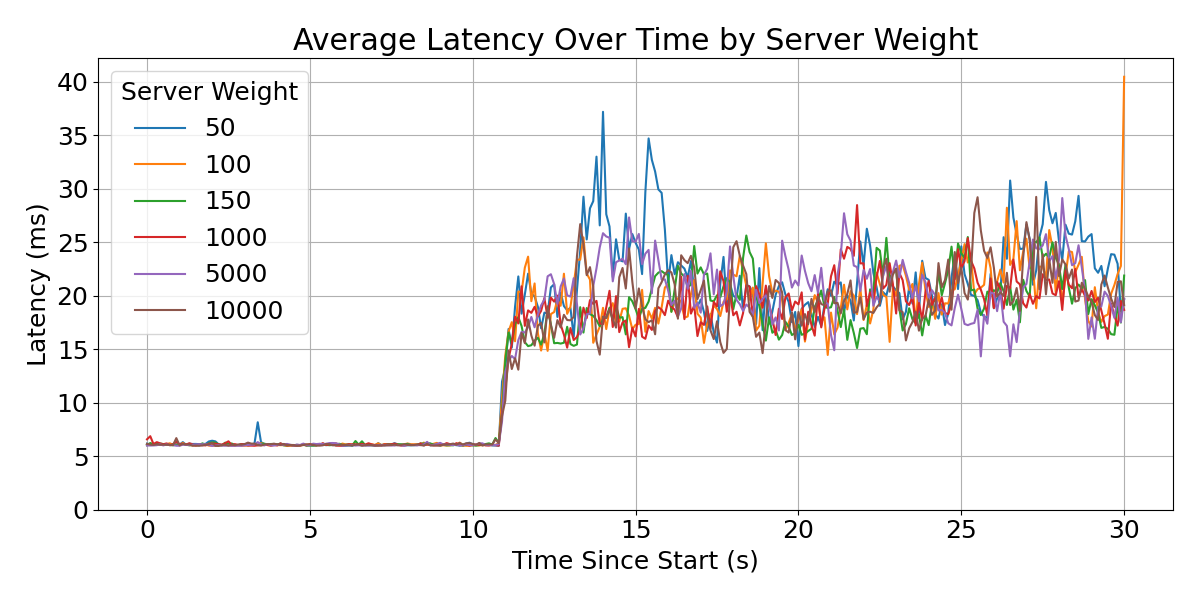
\includegraphics[width=\columnwidth]{graphs/srv-bg-weight-cmp-low.png}
        \caption{Low load, utilization before starting the BE tasks is
        around 85\%}\label{fig:srv-bg-weight-cmp-low}
        \vspace{12pt}
    \end{subfigure}
    \hspace{\fill}
    \begin{subfigure}{\columnwidth}
        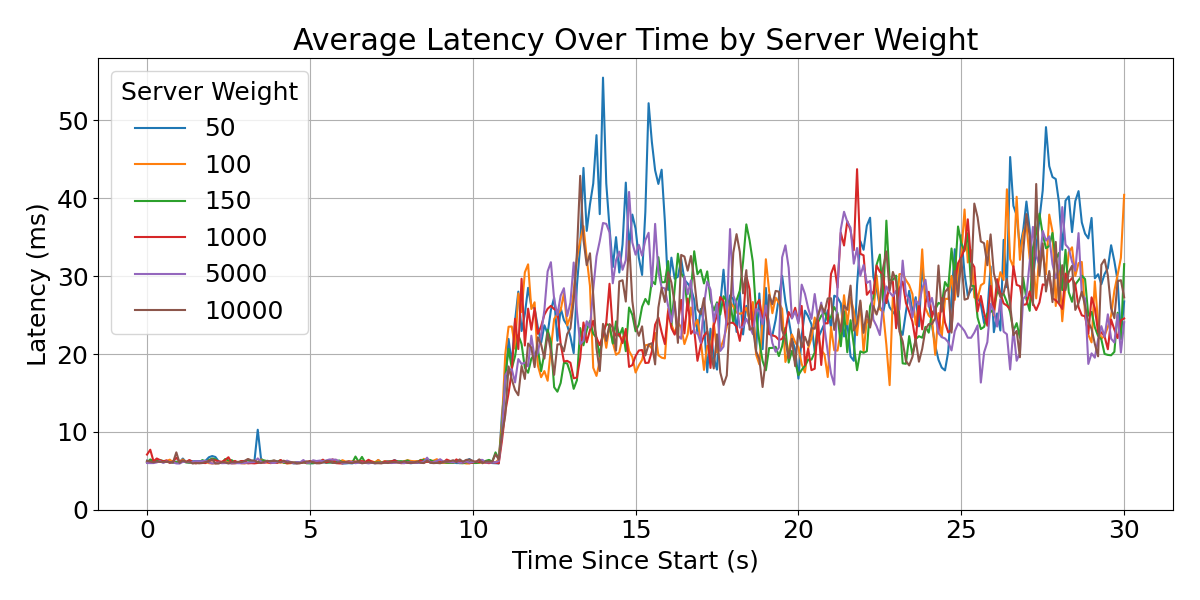
\includegraphics[width=\columnwidth]{graphs/srv-bg-weight-cmp-high.png}
        \caption{High load, utilization before starting the BE tasks is around
        95\%}\label{fig:srv-bg-weight-cmp-high}
    \end{subfigure}
    \vspace{4pt}
    \caption{Changing the weight of the server has little impact on how much the
    weight 1 BE task interferes with it}\label{fig:srv-bg-weight-cmp}
\end{figure}


A simplified experiment shows that \cgroups{} weights are unable to enforce
reservations. We run an open-loop client on a remote machine, and then start two
best effort workloads doing image resizing. We put the LC server and the BE
resize job each in their own group, and pin them to the same four cores.
\cgroups{} supports weights in the range of [1,10000],
\autoref{fig:srv-bg-weight-cmp} shows that running the server with different
weights has no effect on the latency impact of the BE task.

\begin{figure}[t]
    \centering
    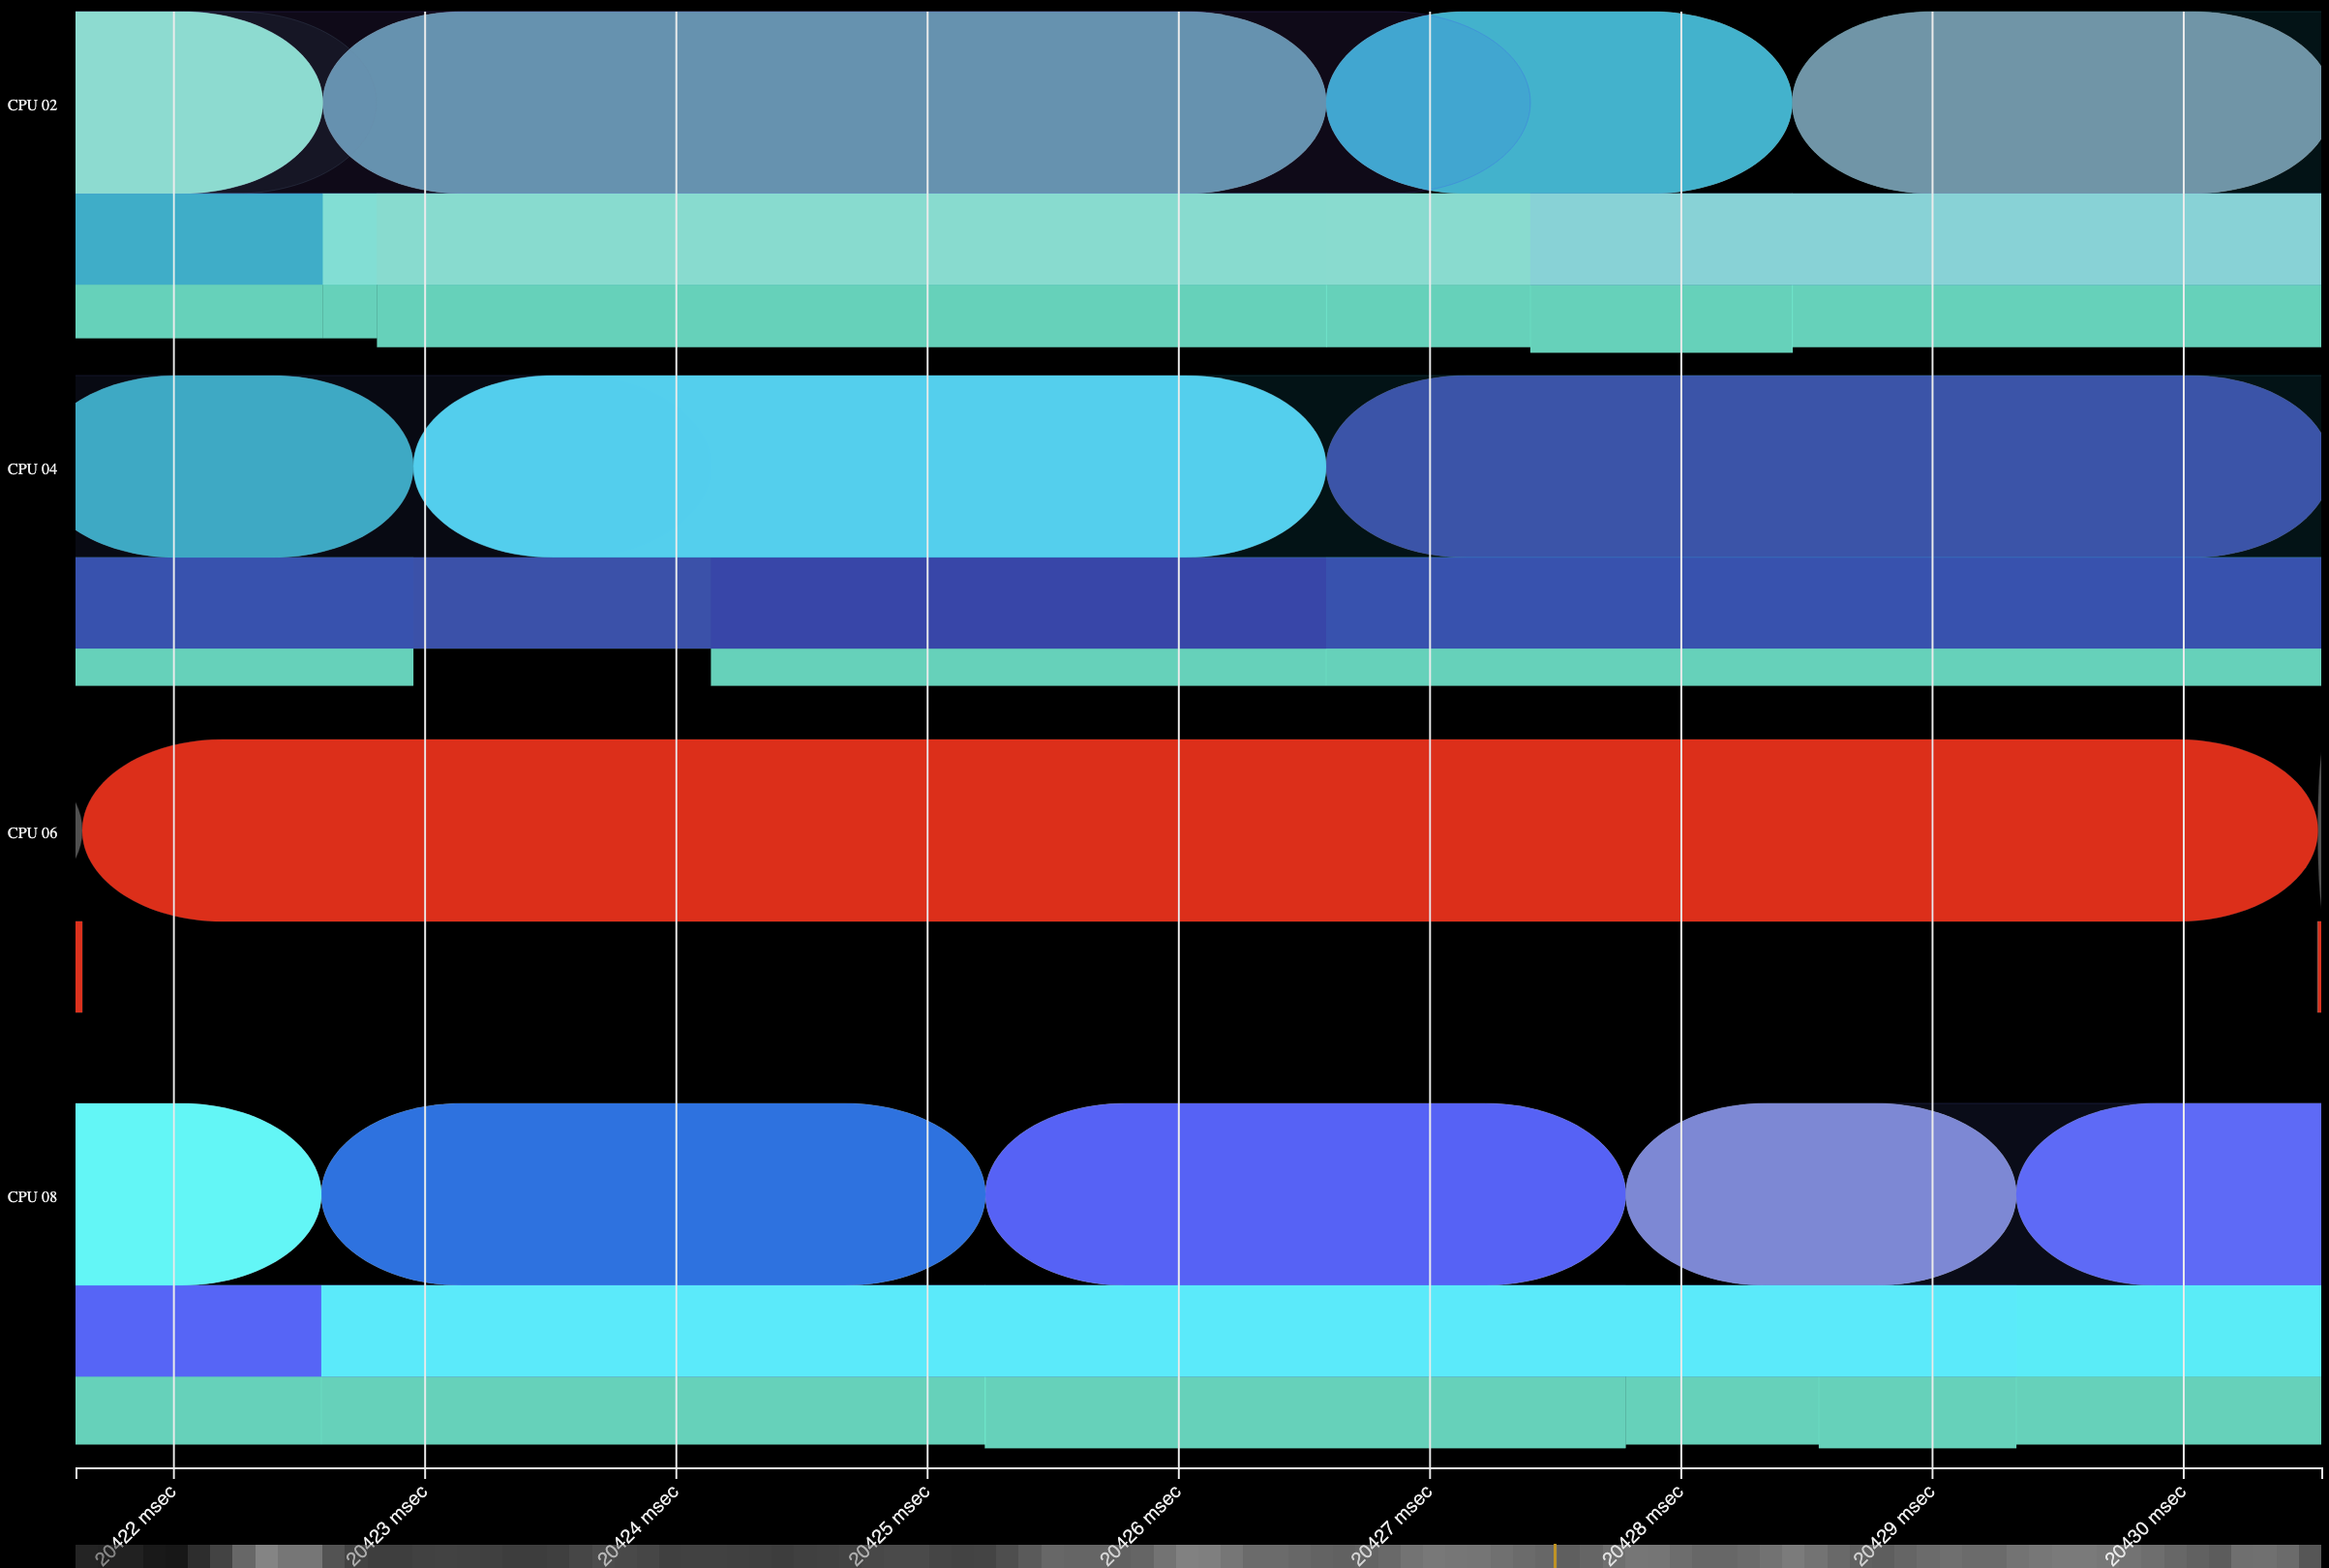
\includegraphics[width=\columnwidth]{graphs/schedviz-problem.png}
    \caption{Core 6 runs an image resize process, unaware that cores 2, 4, and 8
    all have runnable and queued server threads}\label{fig:schedviz-problem}
\end{figure}

The spike in latency after starting the BE happens because the BE sometimes runs
uncontended on one core, even while another has queued and waiting server
threads. \autoref{fig:schedviz-problem} shows an outtake from the trace, where
on core 6, the red process that is running for the whole 10ms is a thread of the
BE job, while server threads, shown in varying shades of blue, are queued on the
other cores.

This priority inversion happens because weights are only enforced within
runqueues, which are per-CPU. Although load balancing eventually remedies this,
it runs less frequently than scheduling does. For sharing across long-running
processes, balancing occasionally works well, but for workloads with runtimes in
the ms, these delays significiantly influence final processing times.

In order to globally enforce weights, each scheduling decision would require a
global search for the process that should be run next. We conclude that weights
are the wrong interface to use to honor reservations globally.




